\documentclass{article}

\usepackage{fancyhdr}
\usepackage[parfill]{parskip}
\usepackage{cite}
\usepackage{hyperref}
\usepackage{graphicx}

\pagestyle{fancyplain}

\author{Todd Davies}
\title{COMP10120: Professional Issues - Intellectual Property}
\date{\today}

\begin{document}

\rhead{COMP10120: Professional Issues - Intellectual Property}
\lhead{\today}

\maketitle

\section{Copyright}

\subsection{What is Copyright?}
Copyright is a legal concept that attempts to give the creators of a wide variety of material economic rights pertaining to the material they've created. \cite{govukwhatis}

\subsection{How is Copyright obtained?}
In the UK, copyright protection is automatic; there's no official registration. When a creator produces an applicable work, the work is automatically protected by copyright. \cite{govukautoprotect}

\subsection{What can Copyright be applied to?}
There are lots of different types of 'material' that can be protected by copyright, including but not limited to music, art, literature, photographs and of course the source code of software. A specific piece of material that is protected by copyright is called a 'work'.

\subsection{Where is Copyright valid?}
The UK has signed the Berne Convention, and thus your copyright is valid in any other country that has also signed the Berne Convention \cite{berneconvention}. These countries include all western European countries, the USA and Russia. \cite{govukabroad}

\subsection{How is Copyright enforced?}
Copyright, in the UK can be enforced in a court, but it is advised that the matter is attempted to be solved through dialog between the involved parties, since this will avoid potential legal fees. \cite{govukenforce}

\section{Who owns and work that I do while I'm studying at The University of Manchester?}

There are many resources produced by the University of Manchester to help both students and staff find information about the ownership of Intellectual Property (IP) that is created while they are at the University.

I've included a particularly relevant image in Figure~\ref{fig:IPOwnership} outlines exactly who IP belongs to when a student does work at the University.

\begin{figure}[h]
\centering
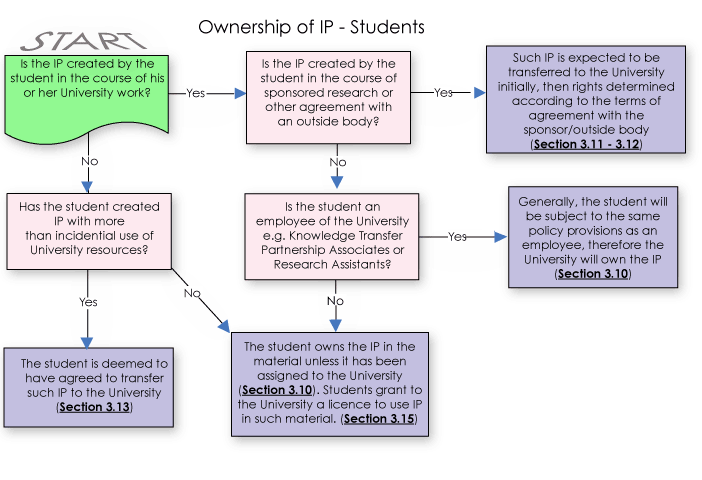
\includegraphics[width=1\textwidth]{IP-ownership-students}
\caption{Ownership of IP}
\label{fig:IPOwnership}
\end{figure}

The University of Manchester has a number of services dedicated to managing IP. One of these is University of Manchester Intellectual Property (UMIP\cite{umip}) which is dedicated to identifying, protecting and evaluating the commercial potential for the University's intellectual property.

The University guide on IP can be found on the University document store (\url{http://documents.manchester.ac.uk/DocuInfo.aspx?DocID=487}).

\begin{thebibliography}{9}

\bibitem{govukwhatis}
  \url{http://www.ipo.gov.uk/types/copy/c-about/c-about-faq/c-about-faq-whatis.htm}

\bibitem{govukautoprotect}
  \url{http://www.ipo.gov.uk/types/copy/c-about/c-about-faq/c-about-faq-automatic.htm}

\bibitem{berneconvention}
  \url{http://en.wikipedia.org/wiki/Berne_Convention_for_the_Protection_of_Literary_and_Artistic_Works}

\bibitem{govukabroad}
  \url{http://www.ipo.gov.uk/types/copy/c-abroad.htm}

\bibitem{govukenforce}
  \url{http://www.ipo.gov.uk/types/copy/c-manage/c-manage-faq/c-manage-faq-howenforce.htm}

\bibitem{umip}
  \url{http://umip.com/}

\end{thebibliography}

\end{document}
